\documentclass[tikz,border=0 4pt 0 0]{standalone}

\usepackage{bm}
\usepackage{tikz}
\usepackage{inter}
\usetikzlibrary{arrows.meta, positioning}

\usepackage{xcolor}
\definecolor{myred}{rgb}{0.8,0.1,0.2}
\definecolor{myblue}{rgb}{0.1,0.2,0.6}
\definecolor{relaxationblue}{RGB}{82,124,197}
\definecolor{quantumblue}{RGB}{145,169,211}
\definecolor{variationalblue}{RGB}{216,225,240}

\begin{document}

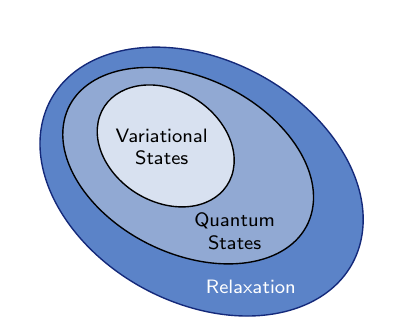
\begin{tikzpicture}[
  scale=1,
  xscale=1.2,
  yscale=1.6,
  every node/.style={font=\sffamily\fontsize{7pt}{8pt}\selectfont},
  line join=round
  ]
  \begin{scope}[rotate=-15]
    \path[fill=relaxationblue, draw=myblue!80!black, line width=0.5pt, fill opacity=0.95]
    (0,0) ellipse [x radius=1.75cm, y radius=1cm];
    \path[fill=quantumblue, draw=black, line width=0.5pt]
    (-0.17cm,0.085cm) ellipse [x radius=1.36cm, y radius=0.72cm];
    \path[fill=variationalblue, draw=black, line width=0.5pt]
    (-0.44cm,0.175cm) ellipse [x radius=0.74cm, y radius=0.46cm];
    \node[align=center] at (-0.48cm,0.16cm)
    {Variational\\States};
    \node[align=center] at (0.44cm,-0.29cm)
    {Quantum\\States};
    \node[text=white] at (0.72cm,-0.67cm)
    {Relaxation};
  \end{scope}
\end{tikzpicture}

\end{document}